\chapter[SCP-176 可见时间循环]{
    SCP-176 Observable Time Loop\\
    SCP-176 可见时间循环
}

\label{chap:SCP-176}

\begin{figure}[H]
    \centering
    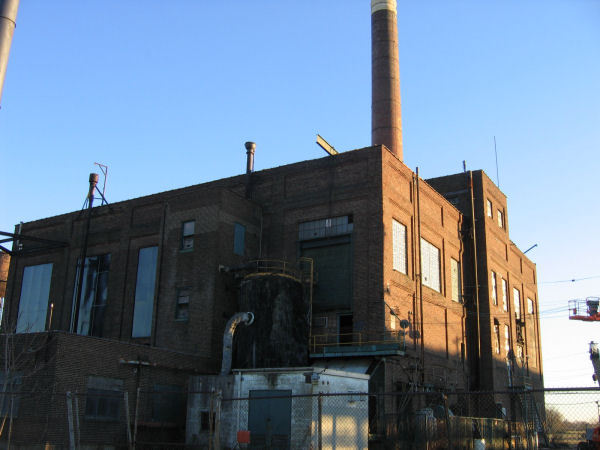
\includegraphics[width=0.5\linewidth]{images/SCP-176.jpg}
    \caption*{SCP-176}
\end{figure}

\bb{项目编号:}SCP-176

\bb{项目等级:}Euclid

\bb{特殊收容措施:}SCP-176以工业化学品污染为掩饰就地收容。任何尝试进入SCP-176的市民必须被拘留。

多个高速摄像机已设置在观测室内并持续连接到运行中的分析计算机上。如果在已记录的序列中出现任何偏差,所有已记录的数据必须立即备份且向高级人员汇报。

\bb{描述:}SCP-176是一座位于{[}数据删除]附近的废弃化工厂。该建筑由一扇工厂门及一个位于二楼,被单面镜从大堂隔开的观测室组成。有着以下三个通往该建筑的入口:

\begin{itemize}
\item 一个有着三个船位的装卸码头,门已经被焊上封死。
\item 位于底层的员工入口。
\item 一个二楼观测室的入口,通过一个位于建筑北方的金属楼梯间进入。
\end{itemize}

当通过装卸码头或员工入口进入主楼时,没有观测到任何异常现象,只有一个已经停用已久并且年久失修的房间,当中有一些金属碎片,完全符合一个倒闭并且废弃了的工厂的形象。通往观测室的楼梯间消失了并且不能通过,而且到目前为止所有从工厂内部门窗进入观测室的尝试均以失败告终。

当通过二楼外面的门进入观测室时,可以看到一个工厂观测室,和建筑其余部分一样停用已久且年久失修。可是,当通过观测室的窗户观看工厂内部时,就可以看到SCP-176的异常性质。

从观测室窗口看到的景象表现出一个固定、重复的场景,一次持续大约11.3秒。从窗户看进去只是一个与工厂的摆设是一样且位于同一维度的房间,但是刷上了白色的漆并且经过了除菌处理。在房间中央设置着一部巨大的、作用不确定的电子设备,占地大约50平方米,最高处约高2米。五名穿着白色干净衣服的人似乎在设备周围工作着。

场景进行大约5.9秒后,员工入口会自行爆开,四名穿着黑色战术装甲、身上没有可辨识的记号或标志的人会进入房间,并向研究人员开火。在11.3秒时, 房间中心的设备放出强烈的闪光和辐射,然后场景重放。对数以千计场景序列的分析没有发现序列的改变。

到目前为止,所有与场景互动的尝试均已失败;任何在观测室内破坏门窗的尝试都会遇到与这些构成门窗框的材料本应拥有的阻力不相符的强大阻力阻挠。迄今为止, 所有成功穿透门窗的尝试,均导致其造成的伤害在序列进行到光芒爆发时被立即彻底修复。所有延伸到观测室外面的工具或边缘均被干净利落地截断了,且不能再被找到。

研究集中于对SCP-176中央设备性质的调查,除此之外还包括里面个体的身份调查。

\bb{附录 176-1:}对SCP-176内个体的进一步分析

关于场景内的可见个体,已经得出以下分析结果:

\begin{itemize}
\item \bb{无法识别身份的研究员\#1:}雄性高加索裔,大约40岁,长着褐色头发和绿色的眼睛。站在房间的东南角,在阅读一个直立显示器上面的信息。在大约8.1秒时肩部被自动枪械射中了三枪,并似乎即时死亡。
\item \bb{无法识别身份的研究员\#2:}雄性亚裔,大约35岁, 长着黑色头发和褐色的眼睛。站在研究员\#1的左边,拿着一个附有纸夹的笔记板,上面的字难以辨认。他在8.0秒时右肩中了一枪并跌倒在设备后面的地上,不能被看到。
\item \bb{无法识别身份的研究员\#3:}雌性高加索裔,大约40岁,长着褐色头发和琥珀色的眼睛。坐在房间西南角的一张书桌前,在电脑台上工作。在枪战开始时就脱离了视线,并躲在书桌下。似乎在序列结束前不久拿到了某种武器。
\item \bb{无法识别身份的研究员\#4:}雄性高加索裔,大约45岁,长着褐色头发和不能看出颜色的眼睛。他站在设备东北方的前面,背对着观测室。在7.2秒时头部中了两枪,即时死亡。
\item \bb{无法识别身份的研究员\#5:}雄性,特征不明。站在西北角,身体大半模糊看不清。推测在7.8秒时被射中并跌倒,跌出视野之外。
\item \bb{无法识别身份的袭击者\#1:}雄性,特征不明,使用一把消音型M4A1。他第一个进入,枪击了研究员\#4和研究员\#5,然后向着该设备移动。
\item \bb{无法识别身份的袭击者\#2:}雄性,特征不明,使用一把消音型MP5N。他第二个进入,左转并枪击了研究员\#1和研究员\#2,然后迅速往东南方前进。
\item \bb{无法识别身份的袭击者\#3:}雄性,特征不明,使用一把消音型MP5N。他第三个进入, 右转并往观测室下移动。
\item \bb{无法识别身份的袭击者\#4:}雄性,特征不明,使用一把消音型TMP。停留在门边,掩护其余队员。
\end{itemize}
